%!TEX root = ../my_thesis.tex
\chapter{Caractérisation, identification et correction des erreurs résiduelles} % (fold)
\chaptermark{Caractérisation, identification et correction des erreurs rés\ldots}
Ce chapitre troisième vise à présenter une méthode permettant de corriger les erreurs résiduelles rencontrées dans la zone
du plancher d'erreurs lors du décodage des turbo codes.

Suite à une observation de ces erreurs grace à des simulations Monte-Carlo, une prédiction de leurs distributions basée sur la borne de l'union est proposée. 
Ceci permet alors de les caractériser.

Dans un second temps, plusieurs critères d'identification de la position de ces erreurs sont proposés et comparés. Ceux-ci 
sont aussi bien adaptés aux turbo codes binaires qu'aux double binaires.

Ceci mène alors à la proposition d'un algorithme permettant de corriger les erreurs résiduelles des turbo codes.
Il a pour propriété d'abaisser drastiquement le plancher d'erreurs lors du décodage des turbo codes.
Une comparaison avec l'état de l'art met en exergue l’intérêt de cette approche.


\vspace*{\fill}
\minitocTITI
\vspace*{\fill}
\newpage

\section{Analyse des erreurs résiduelles}
\subsection{Caractérisation théorique}
Comme présenté dans le premier chapitre, l'apparition du plancher d'erreurs dépend de la distribution des mots de codes 
possédant un faible poids \cite{distance_spectrum}. Plus encore, il a été montré que la zone du plancher d'erreurs émanait 
de la présence \emph{d'erreurs résiduelles} \cite{takeshitaBCH}. 
La Figure \ref{fig:befe} présente l'évolution du nombre moyen de bits erronés par trame erronée en fonction de la valeur de 
SNR pour six turbo codes binaires différents. Cinq de ces codes appartiennent au standard LTE, le cinquième au standard CCSDS. 
À chaque fois, un rendement de 1/3 et un turbo décodage basé sur l'algorithme EML-MAP itérant 8 fois sont considérés. Dans la zone de 
convergence, de nombreuses erreurs sont présentes  à l'issu du décodage. En revanche, dès lors que le décodeur 
fonctionne dans la zone du plancher d'erreurs, le nombre moyen d'erreurs binaires par trame erronée est inférieur à 10. 
De là vient leur nom d'erreurs résiduelles.

\begin{figure}[!b]
	\centering
	\includegraphics[width=.8\textwidth]{main/ch3_fig/be/tikz/befe.pdf}
	\caption{Évolution du nombre moyen d'erreurs binaires par trame erronée pour différentes valeurs de SNR et différents
	turbo codes. Décodage effectué par l'algorithme EML-MAP itérant 8 fois. \label{fig:befe}}
\end{figure}

Une caractérisation de la distribution de ces erreurs 
résiduelles a été proposée dans \cite{residual_errors}. Cette dernière est basée sur les fonctions recenseuses de poids
(Weight Enumerator Functions ou WEF en anglais, \cite{ryan}). En posant $P^{\langle ML\rangle}(m)$ la probabilité que 
$m$ bits soient erronés dans une trame et sachant que la trame est erronée après un décodage à maximum de vraisemblance,
l'expression suivante est obtenue :
\begin{equation}
P^{\langle ML\rangle}(m) \simeq \frac{W^m~A_m^{\langle CP\rangle}(Z)\vert_{W=Z=e^{-RE_b/N_0}}}{\sum\limits_{w=1}^N W^w~A_w^{\langle CP\rangle}(Z) \vert_{W=Z=e^{-RE_b/N_0}}}
\label{eq:be1}
\end{equation}
où $A_w^{\langle CP\rangle}(Z)$ est le WEF conditionnel du turbo code considéré \cite{benedetto_unveiling}.

En supposant que les séquences d'information 
générant un mot de code de poids $w$ ont majoritairement le même poids, l'équation précédente peut alors être transformée 
en : 
\begin{equation}
P^{\langle ML\rangle}(m) \approx \frac{\displaystyle\sum\limits_{w, \frac{W_w}{A_w}=m} A_w\cdot \exp\left(-w R \frac{E_b}{N_0}\right)}
                  {\displaystyle\sum\limits_{w} A_w\cdot \exp\left(-w R \frac{E_b}{N_0}\right)}
\label{eq:be2}
\end{equation}
avec, comme déjà introduit dans le premier chapitre, $A_w$ le nombre de mots de code de poids de Hamming $w$. La 
multiplicité des bits d'information $W_w$ est la somme des poids de Hamming des $A_w$ séquences binaires générant des
mots de code de poids de Hamming $w$. Au prix d'une faible imprécision, cette forme de l'équation permet d'utiliser 
directement le spectre de distances d'un turbo code pour estimer le nombre de bits erronés dans le plancher d'erreurs. Les
résultats obtenus avec cette équation différent alors légèrement de ceux obtenus avec l'Équation \ref{eq:be1}. En effet,
certaines valeurs sont masquées par l'opération de moyenne : $\frac{W_w}{A_w}=m$. 

Ainsi, le spectre de distances d'un turbo code permet de calculer la probabilité 
d'obtenir $m$ erreurs binaires dans une trame erronée en considérant un décodage ML pour un taux d'erreur suffisamment 
faible et un canal AWGN. De part la présence du terme en exponentielle, plus le poids du mot de code $w$ est distant 
de $d_{min}$, moins la multiplicité associée a un impact sur la distribution des erreurs résiduelles. Ceci peut néanmoins
être fortement atténué par une multiplicité très importante (de l'ordre du millier, rencontré fréquemment lors des 
expérimentations).

% Dans la section suivante, grâce à l'obtention des spectres de distances de différents turbo codes standardisés, une 
% comparaison est menée quant à la distribution du nombre d'erreurs dans les trames erronées dans la zone du plancher 
% d'erreurs.
Dans la section suivante, ces résultats théoriques sont comparés à des distributions observées du nombre d'erreurs binaires dans les
trames erronées de la zone du plancher d'erreurs avec un décodage basé sur l'algorithme ELM-MAP.

\subsection{Observations considérant des turbo codes standardisés}
Une méthode proposant de prédire théoriquement la distribution des erreurs résiduelles dans la zone du plancher d'erreurs 
a été  établie. L'obtention 
de la distribution réelle de ces erreurs est maintenant réalisée et elle est comparée avec cette méthode. Dans un premier 
temps, des turbo codes binaires de tailles de 
trames différentes et de rendement 1/3 sont considérés. Dans un second temps, des turbo codes double binaires de deux
tailles de trame mais de différents rendements sont considérés. Ainsi, un large spectre de paramètres est exploité sans
présenter un nombre trop conséquent de données.

\subsubsection{Dans le cas de turbo codes binaires}
\begin{figure}[!ht]
	\centering
	\hspace*{-1cm}
	\includegraphics[width=1.07\textwidth]{main/ch3_fig/be/tikz/be.pdf}
	\caption{Distribution du nombre d'erreurs binaires pour différentes valeurs de SNR et différents turbo codes des 
	standards LTE et CCSDS. 
	Décodage EML-MAP itérant 8 fois. \label{fig:be}}
\end{figure}

La Figure \ref{fig:be} présente la distribution des erreurs résiduelles pour 5 turbo codes du standard LTE et un du 
standard CCSDS. Le rendement du code est fixé à 1/3. Pour chacun de ces histogrammes, 500 trames erronées
après décodage via l'algorithme EML-MAP itérant 8 fois sont considérées. 
Pour chacun des turbo codes, trois valeurs de SNR sont présentées. La première correspond à un fonctionnement du turbo 
code dans la zone de convergence. La seconde valeur correspond au point d'inflexion de la courbe de performance et la troisième à la
zone du plancher d'erreurs. Conformément aux résultats de la Figure \ref{fig:befe}, lorsque la valeur de SNR augmente, la 
distribution des erreurs se concentre sur de faibles nombres d'erreurs binaires.
Il apparaît alors que pour la troisième valeur de SNR, la très grande majorité 
des trames erronées contiennent moins de 10 erreurs binaires. 
%Ceci est conforté par la Figure \ref{fig:befe}. 
Plus encore, hormis pour le turbo code du standard CCSDS, 70\% des trames erronées ont strictement moins de 5 erreurs.

Sont aussi présentés sur la Figure \ref{fig:be} les résultats théoriques obtenus pour la valeur de SNR la plus grande
grâce à l'équation \ref{eq:be1} et au spectre de distances calculé via la Double Impulse Method (cf. \ref{seq:spectre}). 
Les spectres de distances de ces différents turbo codes sont présentées en Annexe \ref{sec:ann3}. Les distributions théoriques
calculées sont reportées pour plus de lisibilité dans le Tableau \ref{tab:theo}. Suivant le turbo code considéré,
des différences entre la valeur théorique et la valeur mesurée apparaissent. Néanmoins, la tendance pour les valeurs
calculées est conforme
aux mesures obtenues. Ainsi, la seule occurrence non prédite correspond à un seul bit erroné pour le standard CCSDS, où $0,2\%$ 
était prédit alors que $11\%$ sont mesurés. Cette observation trouve un explication dans la sous-optimalité du décodage 
itératif des turbo codes, discuté plus loin.

\begin{table}[]
\centering
\caption{Distribution théorique des erreurs dans le plancher d'erreurs selon l'équation \ref{eq:be1} pour différents turbo 
codes standardisés}
\label{tab:theo}
\resizebox{\textwidth}{!}{
\begin{tabular}{@{}lrrrrrrrrrrr@{}}
\toprule
                            & 1      & 2      & 3      & 4      & 5     & 6      & 7     & 8      & 9     & 10  & \textgreater10 \\ \cmidrule(r){1-1} \cmidrule(l){2-12}
LTE R=1/3, K=528 @ $2,4$ dB    & $33,9\%$ & $24,4\%$ & $29,3\%$ & $1,4\%$  & $1\%$   & $5,2\%$  & $0,2\%$ & $0,02\%$ & $4,6\%$ & 0\% & 0\%            \\
LTE R=1/3, K=1024 @ $1,5$ dB   & $19,9\%$ & $32,7\%$ & $36,7\%$ & $6,2\%$  & $3,6\%$ & $0,3\%$  & $0,4\%$ & $0,2\%$  & $0\%$   & 0\% & 0\%            \\
LTE R=1/3, K=1504 @ $1,3$ dB   & $0\%$    & $19,2\%$ & $68\%$   & $8,3\%$  & $2,2\%$ & $0,8\%$  & $1,4\%$ & $0\%$    & $0\%$   & 0\% & 0\%            \\
LTE R=1/3, K=2048 @ $1,3$ dB   & $26\%$   & $33,7\%$ & $30,2\%$ & $7,9\%$  & $1,4\%$ & $0,3\%$  & $0,4\%$ & $0,1\%$  & $0\%$   & 0\% & 0\%            \\
LTE R=1/3, K=6144 @ $0,8$ dB   & $0\%$    & $76\%$   & $7,2\%$  & $14,2\%$ & $2,1\%$ & $0,3\%$  & $0,1\%$ & $0\% $   & $0\%$   & 0\% & 0\%            \\
CCSDS R=1/3, K=1784 @ $1,3$ dB & $0,2\%$  & $48,1\%$ & $27,9\%$ & $0,2\%$  & $0,1\%$ & $22,3\%$ & $0,1\%$ & $0,1\%$  & $0,6\%$ & 0\% & 0\%            \\ \bottomrule
\end{tabular}}
\end{table}

Afin de présenter la déviation entre la théorie développée dans la première section de ce Chapitre et les mesures 
effectuées, un calcul d'erreur quadratique moyenne (EQM, Équation \ref{eq:eqm}) est effectué pour chacun des turbo codes. 
Les valeurs obtenues sont récapitulées dans le tableau \ref{tab:eqm}.

\begin{equation}
	EQM = \sqrt{\cfrac{1}{N}\sum\limits_{i=1}^N\bigl(T_i-M_i\bigr)^2} \text{~~avec~~} \begin{cases}
		T_i \text{~~la valeur théorique} \\
		M_i \text{~~l'observation}
		\end{cases}
	\label{eq:eqm}
\end{equation}

Les valeurs d'EQM sont alors comprises entre $3,8$ et $9,5$, impliquant que les valeurs théoriques et mesurées sont 
relativement proches. Ainsi même si des écarts apparaissent, ces équations permettent de prédire l'allure de la distribution
des erreurs binaires dans la zone du plancher d'erreurs. Les écarts s'expliquent par le fait que les Équations \ref{eq:be1} 
et \ref{eq:be2} ne sont vraies que dans le cas d'un décodage ML. Or ce dernier ne peut pas être effectué dans le contexte 
des turbo codes en raison de la complexité calculatoire. Il semble alors apparaître que le décodage EML-MAP entraîne un 
étalement des valeurs vis-à-vis de celles théoriques n'étant vraies que pour un décodage ML.

Plus le ratio $\frac{W_d}{A_d}$ des premiers termes du spectre de distances du code est faible, plus le nombre moyen de 
bits erronés par trame erronée dans le plancher d'erreurs sera faible lui aussi. Pour les turbo codes 
standardisés, les ratios $\frac{W_d}{A_d}$ sont habituellement faibles. Ceci implique alors une distribution des erreurs 
binaires dans le plancher d'erreurs centrée sur les faibles nombres d'erreurs.
\begin{table}[t]
\centering
\caption{Erreur quadratique moyenne entre les valeurs théoriques et les simulations Monte-Carlo}
\label{tab:eqm}
\vspace*{-1em}
\resizebox{.4\textwidth}{!}{
\begin{tabular}{@{}lr@{}}
\toprule
                            & EQM \\
                      \cmidrule(r){1-1}      \cmidrule{2-2}
LTE R=1/3, K=528    @ $2,4$ dB & $6,2$ \\
LTE R=1/3, K=1024   @ $1,5$ dB & $9,4$ \\
LTE R=1/3, K=1504   @ $1,3$ dB & $9,5$ \\
LTE R=1/3, K=2048   @ $1,3$ dB & $3,8$ \\
LTE R=1/3, K=6144   @ $0,8$ dB & $6,7$ \\
CCSDS R=1/3, K=1784 @ $1,3$ dB & $6,9$ \\
\bottomrule
\end{tabular}}
\end{table}

Maintenant, une analyse similaire vient confirmer et étendre ces résultats dans le contexte de turbo codes double binaires.

\subsubsection{Dans le cas de turbo codes double binaires}
Dans le contexte de turbo codes double binaires, deux analyses complémentaires sont nécessaires. En effet, en plus du 
nombre d'erreurs binaires (noté BE), le nombre d'erreurs symboles (noté SE) peut être aussi comptabilisé. Par définition, 
le nombre d'erreurs symboles est compris entre $\frac{\text{BE}}{2} $ et $\text{BE}$. En effet, si un bit d'un symbole 
est erroné, alors le symbole est lui même erroné. Mais, un symbole erroné se compose d'un ou deux bits erronés.

Les méthodes d'obtention du spectre de distances telles que la Double Impulse Method permettent de calculer la multiplicité 
des bits d'information ($W$). Par extension, il est aussi possible de calculer la multiplicité des symboles d'information
($W^S$). En considérant l'équation \ref{eq:be2}, la probabilité que $m$ symboles soient erronés dans une trame sachant 
que la trame est erronée après un décodage ML a pour expression: 
\begin{equation}
P_S^{\langle ML\rangle}(m) \approx \frac{\displaystyle\sum\limits_{w, \frac{W^S_w}{A_w}=m} A_w\cdot \exp\left(-w R \frac{E_b}{N_0}\right)}
                  {\displaystyle\sum\limits_{w} A_w\cdot \exp\left(-w R \frac{E_b}{N_0}\right)}
\label{eq:se}
\end{equation}
La Figure \ref{fig:be_dvb440} présente la distribution des erreur binaires et symboles pour différents turbo codes du 
standard DVB-RCS avec K=440 symboles et différents rendements allant de R=1/3 à R=6/7. Le processus de décodage est réalisé par
l'algorithme EML-MAP itérant 8 fois où le facteur de remise à l'échelle vaut $0,5$ pour les deux premières itérations et $0,85$ 
au cours des itérations suivantes. 100 trames erronées après décodage sont considérées pour les expérimentations. Comme 
dans le cas de turbo codes 
binaires, il apparaît que la très grande majorité des trames contiennent au plus 10 erreurs binaires. En ce qui concerne 
le nombre d'erreurs symboles, la distribution est semblable mais décalée vers la gauche de 0 à 3 erreurs suivant le turbo 
code considéré. Ceci est conforme avec le fait qu'une erreur symbole corresponde à 1 ou 2 erreurs binaires. 

\begin{figure}[!h] 
	\centering
	\hspace*{-1cm}
	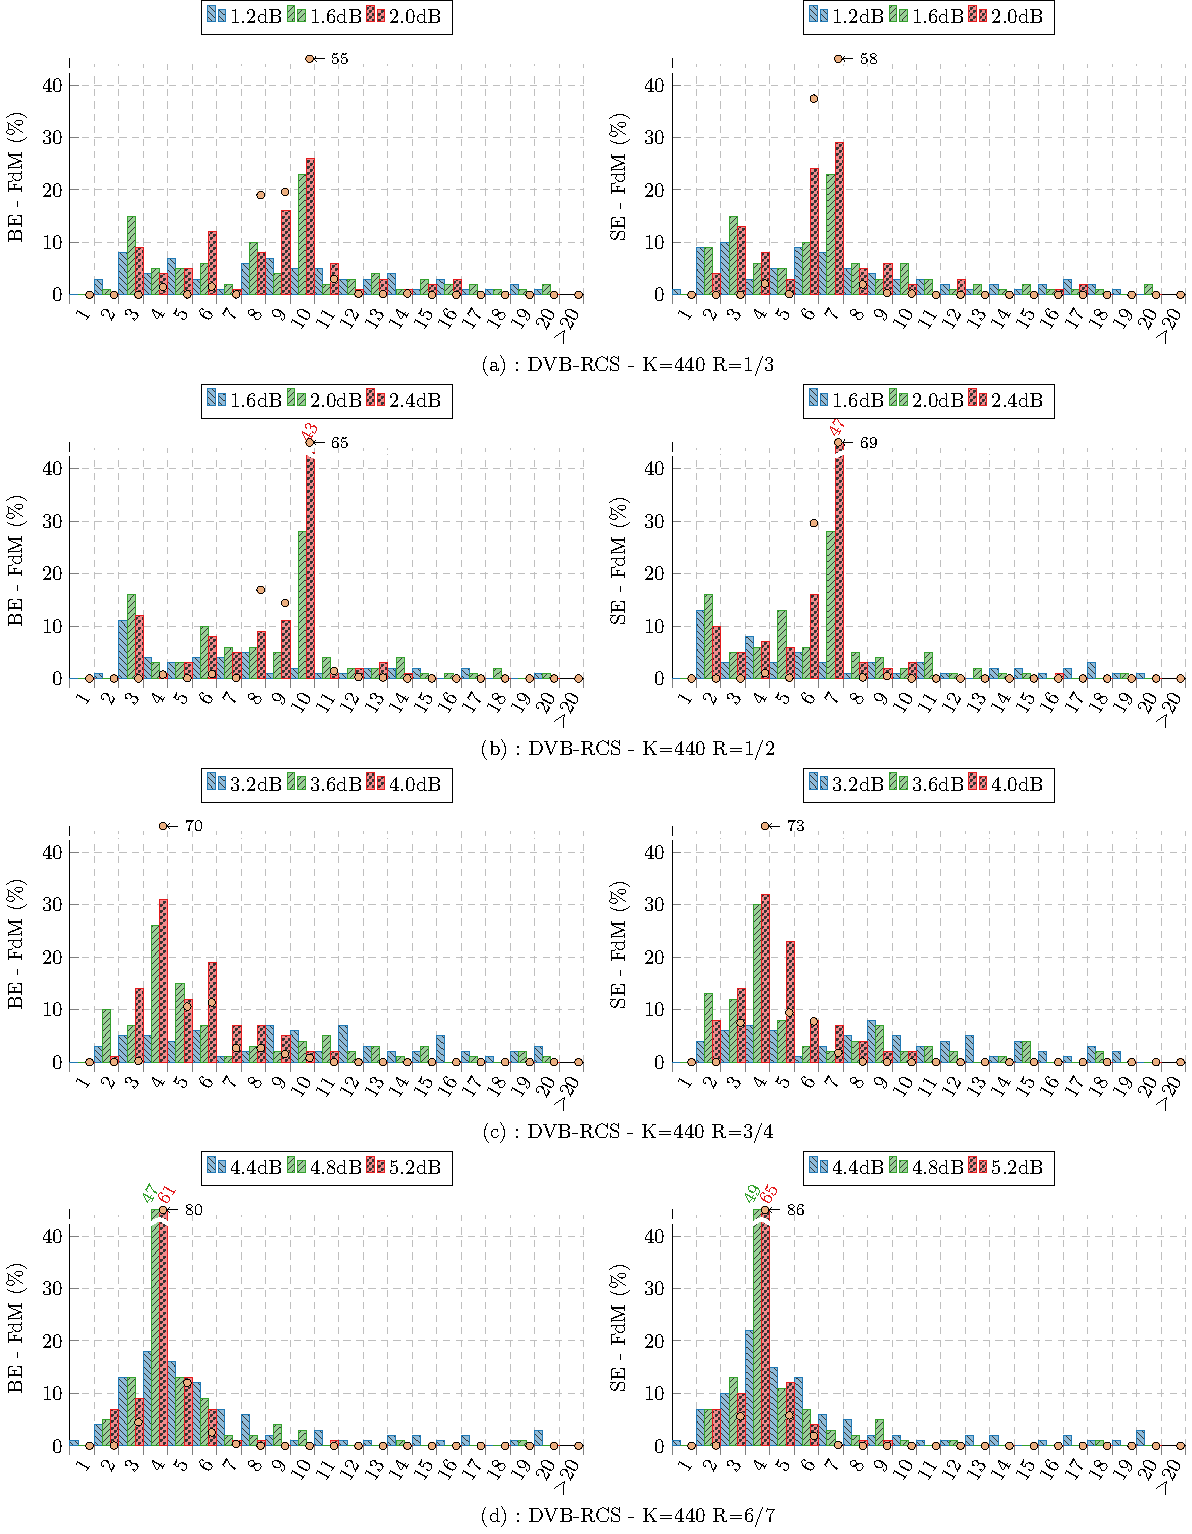
\includegraphics[width=1.04\textwidth]{main/ch3_fig/be/dvb/tikz/be_440.pdf}
	\caption{Distribution du nombre d'erreurs binaires et symboles pour différentes valeurs de SNR et pour différents turbo codes du 
	standard DVB-RCS pour K=440.	Décodage EML-MAP itérant 8 fois. \label{fig:be_dvb440}}
\end{figure}

Afin de comparer ces données expérimentales avec des valeurs théoriques, l'équation \ref{eq:se} est utilisée avec les 
spectres de distances obtenus grâce à la méthode DIM pour les différents turbo codes. Ces spectres de distances sont 
présentés en Annexe \ref{sec:ann3}. Les résultats théoriques sont calculés en considérant la valeur de SNR la plus élevée 
considérée pour les simulations et sont reportés sur la Figure \ref{fig:be_dvb440}. Il apparaît alors, qu'à nouveau, les équations
\ref{eq:be2} et \ref{eq:se} permettent de prédire la distribution des erreurs dans la zone du plancher d'erreurs de manière fiable. 
Nous pouvons constater que toutes les valeurs d’occurrence maximale sont correctement prédites que ce soit pour les erreurs binaires ou les 
erreurs symboles. Des écarts apparaissent pour les faibles nombres d'erreurs. Ceci s'explique là encore par la validité des
différents équations dans le cas d'un décodage ML, non réaliste pour des turbo codes de tailles conséquentes.
Ainsi, dans le cas d'un décodage EML-MAP, la distribution observée des erreurs est plus étalée que celle prédite.

La même étude a été menée dans le cas des turbo codes du standard DVB-RCS avec K=752. Les résultats numériques ainsi
que leurs spectres de distances sont fournis en Annexe \ref{sec:ann3} pour des rendements valant 1/3, 1/2, 3/4 et 6/7. 
Ces résultats complémentaires confirment ceux détaillés dans cette sous-section. Ainsi, la prédiction théorique de la distribution des erreurs binaires 
ou symboles est valide ce quelque soit le turbo code considéré. Il peut être binaire ou double binaire, de petite ou grande
taille de trame et à faible ou fort rendement.

Finalement, lorsqu'un processus de décodage itératif échoue au niveau du plancher d'erreurs, la trame résultante est très proche du 
mot de code transmis. Cette constatation semble se réaliser pour tout turbo code standardisé, incluant les turbo codes
double binaires. Dans la section suivante, différents critères d'identification de ces erreurs résiduelles sont 
proposés, évalués et comparés.
\newpage
\section{Comparaison de critères d'identification}
Dans cette section, une comparaison de plusieurs métriques permettant l'identification des positions des erreurs résiduelles est 
proposée. Ces différentes métriques sont basées sur des quantités internes du turbo décodeur qui seront détaillées ci-après.\\
Suite aux résultats obtenus dans le deuxième chapitre des métriques reposant sur des oscillations sont écartées. Ainsi, 
seules des métriques prenant en compte l'amplitude d'informations internes au turbo décodeurs sont privilégiées.

\subsection{Les différentes métriques considérées pour les turbo codes binaires}
Comme nous l'avons vu dans le chapitre précédent, le module de l'information \textit{a posteriori} calculée par le turbo 
décodeur représente le niveau de confiance associé à chaque bit du mot décodé.
Ainsi, une première métrique pouvant 
être établie est la suivante :
\begin{equation}
	\Delta_1(k) = |L^a(k)|\text{~, avec k~}\in \llbracket0;~K \rrbracket 
\end{equation}
%Par ailleurs, il peut être considéré que de décorréler les informations du canal pour la métrique peut être intéressant. 
Par ailleurs, décorréler les informations du canal de la métrique peut s'avérer intéressant.
En effet, 
cela permet d'exprimer seulement l'avis propre au décodeur. Cette métrique est alors uniquement basée sur les informations 
extrinsèques et a pour expression : 
\begin{equation}
	\Delta_2(k) = |L^e_{12}(k)+L^e_{21}(k)|
\end{equation}
D'autre part, il peut être judicieux de considérer une norme au sens mathématique. L'évaluation de la norme 1 
(distance de Manhattan) est suffisante puisque son emploi vise à ordonner des positions. En effet, l'ordre est 
conservé quelque soit la norme p ($p \in \mathbb{N} $) employée. Les expressions des deux équations précédentes deviennent 
alors respectivement :
\begin{equation}
	\Delta_3(k) = |y^s(k)| + |L^e_{12}(k)| + |L^e_{21}(k)|
\end{equation}
et 
\begin{equation}
	\Delta_4(k) = |L^e_{12}(k)| + |L^e_{21}(k)|
\end{equation}

Pour l'ensemble de ces métriques, les positions les moins fiables sont extraites en identifiant les valeurs $k$ minimisant
ces métriques.

\subsubsection{Résultats d'identification}
Afin de comparer ces différentes métriques, des statistiques d'identification vont être exploitées. Le protocole 
expérimental est le suivant. Après chaque itération du processus de turbo décodage, les $q$ positions les moins fiables
dans la trame sont identifiées grâce à chacune de ces métriques. Si l'ensemble des erreurs est présent dans ces $q$ éléments,
alors l'identification est considérée comme réussie. Les turbo codes considérés sont des turbo codes binaires du standard LTE.
Plusieurs valeurs de SNR sont successivement étudiées. Afin 
d'obtenir des données valides, 500 trames erronées après un décodage par l'algorithme EML-MAP itérant 8 fois sont
observées.

La Figure \ref{fig:id1024} présente les résultats pour le turbo code LTE avec K=1024 et R=1/3. Le nombre de positions les moins fiables
considérées $q$ s'étalent de 4 à 20. Chaque sous-figure correspond à une valeur de SNR différente. Il apparaît tout d'abord que 
les deux critères d'identification basés sur une norme ($\Delta_3$ et $\Delta_4$) présentent les moins bonnes performances.
 Ceci peut être interprété en remarquant que les normes ne permettent pas d'identifier les
cas où chaque décodeur possède un avis ferme (forte amplitude) mais différent l'un de l'autre (signes opposés). Les deux 
autres métriques identifient en revanche cette configuration. La même constatation est faite pour d'autres turbo codes. 
Ainsi, l'utilisation d'une norme (au sens mathématique) est écartée dans la suite, ce au profit des métriques $\Delta_1$ 
et $\Delta_2$.

Ces deux dernières possèdent des performances proches avec un avantage pour la métrique $\Delta_1$. Il est à noter que le pouvoir 
d'identification de ces deux métriques augmente lorsque la valeur de SNR augmente. Ceci est corrélé avec la diminution du 
nombre moyen d'erreurs binaires par trame constatée dans la section précédente.

Toujours en considérant la Figure \ref{fig:id1024}, selon la profondeur de recherche employée et pour une valeur de SNR 
de $1,1$ dB, entre 10 et 30\% des trames ont l'ensemble de leurs erreurs binaires identifiées. Ces taux ne 
permettent pas de proposer une correction intéressante. En effet, en supposant que ces 30\% de trames dont les erreurs sont 
identifiées soient effectivement corrigées par un mécanisme basé sur cette métrique, le taux d'erreur trame passerait alors 
de $2,3\times 10^{-4}$ à $1,6\times 10^{-4}$. L'amélioration des performances serait alors toute relative.

En considérant maintenant une valeur de SNR de $1,3$ dB, le taux d'identification maximal atteint 65\% pour $n=20$ avec la 
métrique $\Delta_1$. Le taux d'erreur trame résultant passerait alors de 
$1,5\times 10^{-5}$ à $5,2\times 10^{-6}$. Cette fois, des gains substantiels sont possibles. D'après les données de la 
Figure \ref{fig:be}, dans ce même cas expérimental, 71\% des trames ont 20 erreurs ou moins. 
L'emploi de la métrique $\Delta_1$ semble alors permettre d'identifier l'ensemble des erreurs de 91\% des trames ayant 
moins de 20 erreurs binaires. Ce taux s'établit à 83\% pour la métrique $\Delta_2$. 
%Il apparaît donc que le pouvoir d'identification de ces métriques est important.
%En effet, seules de rares trames à faibles erreurs binaires n'ont pas eu la position 
% de leurs erreurs identifiées. Ainsi, les performances de la métrique sont d'autant plus importantes que le nombre de bits
% erronés par trames erronées est faible. Cette assertion est vérifiée avec la valeur de SNR la plus élevée considérée.
Il apparaît donc que seules de rares trames à faible nombre d'erreurs binaires n'ont pas l'ensemble de leurs erreurs
identifiées. Il est attendu que plus la valeur de SNR augmente, plus le nombre d'erreurs binaires par trame erronée 
baisse. Par conséquent, les métriques identifient encore plus d'erreurs.

Ceci est vérifié, pour une valeur de SNR de $1,5$ dB. Avec une profondeur de recherche fixée à $10$, $87,6\%$ des 
trames erronées ont l'intégralité de leurs erreurs identifiées grâce à la métrique $\Delta_2$. Ce taux atteint $89,4\%$ avec 
la métrique $\Delta_1$. Pour cette valeur de SNR, $93,8\%$ des trames possède 10 erreurs ou moins. Ainsi, les métriques 
permettent une identification quasiment parfaite de la position des erreurs résiduelles. Finalement, si chaque trame 
erronée dont la totalité des erreurs sont identifiées est corrigée, le taux d'erreur trame résultant passe de 
$3,6\times 10^{-6}$ à une valeur comprise entre $3,8\times 10^{-7}$ et $4,4\times 10^{-7}$ suivant la métrique $\Delta_1$ 
ou $\Delta_2$ employée.

\begin{figure}[!htb]
	\centering
	\includegraphics[width=.75\textwidth]{main/ch3_fig/id2/tikz/1024.pdf}
	\caption{Pourcentage d'identification réussie des erreurs résiduelles pour le turbo code du standard LTE K=1024, R=1/3.
	Décodage EML-MAP itérant 8 fois. \label{fig:id1024}}
		%\vspace*{-1cm}
\end{figure}
%\newpage
La Figure \ref{fig:idLTE} présente les statistiques d'identification réussies pour trois autres turbo codes du standard 
LTE. Dans les trois cas considérés, les observations faites lors de l'analyse de la Figure \ref{fig:id1024} sont
vérifiées. Ces histogrammes valident donc la pertinence des métriques $\Delta_1$ et $\Delta_2$ pour l'identification des bits 
erronés lors du processus itératif de décodage. Dans tous les cas, pour des valeurs de SNR correspondant à un fonctionnement des 
turbo décodeurs dans la zone du plancher d'erreurs, au moins 90\% des trames erronées ont l'ensemble de leurs erreurs 
identifiées par la métrique $\Delta_1$ pour un profondeur de recherche de taille 6.

Dans la section suivante, les métriques proposées sont étendues et caractérisées pour des turbo codes double 
binaires. 

\begin{figure}[!h]
	\centering
	%\hspace*{-.7cm}
	\includegraphics[width=1\textwidth]{main/ch3_fig/id2/tikz/lte.pdf}
	\caption{Pourcentage d'identification réussie des erreurs résiduelles pour différents turbo codes du standard LTE K=528, K=2048 et K=6144 avec R=1/3.
	Décodage EML-MAP itérant 8 fois. \label{fig:idLTE}}
\end{figure}

\subsection{Extension des critères d'identification aux turbo codes double binaires}
Le décodage des turbo codes double binaires a été détaillé en section \ref{sec:dbl}. Pour rappel, ce décodage est basé
sur l'échange de 4 valeurs extrinsèques par symbole. En réalité, dans un but de simplification de 
l'architecture matérielle associée, seules trois valeurs sont échangées puisqu'elles sont normalisées vis-à-vis de 
la probabilité d'obtenir le symbole $\mathbf{0}$. 

La généralisation des métriques $\Delta_1$ et $\Delta_2$ au cas double binaire n'est pas triviale. Dans la suite, une 
extension permettant d'atteindre une identification au moins aussi bonne que celle présentée précédemment est décrite.
L'équation de la métrique $\Delta_1$ dans le cas binaire peut être exprimée de la sorte : 
\begin{align*}
\Delta_1(k) &= |L^a(k)|\\
			&= |l^a_0(k)-l^a_1(k)|,
\end{align*}
où $l^a_b(k)$ représente la log-vraisemblance (LL) \textit{a posteriori} que le bit considéré prenne la valeur b, 
c'est-à-dire, 
$l^a_b(k) = log\left(P(\hat{b_k} = b)\right)$. Ceci peut alors être interprété comme la distance entre les deux LLs de chaque 
symbole
binaire possible (0 et 1). L'extension directe au cas double binaire devrait alors considérer le calcul de 6 distances 
analogues puisque le
nombre de symboles est porté à 4 ($\mathbf{0}, \mathbf{1}, \mathbf{2}, \text{~et~} \mathbf{3}$). Une combinaison 
de ces 6 distances serait alors nécessaire pour caractériser chaque symbole avec une valeur scalaire. Cette valeur 
refléterait la fiabilité du symbole considérée. Cependant, de tels calculs s'avèrent complexes à entreprendre. Nous proposons
donc de considérer uniquement les deux symboles les plus probables $S_{M_x}$ et $S_{M_y}$ qui maximisent $l^a_s$ :
% \begin{align*}
% S_{M_x}(k) &= \argmax\limits_{s\in\llbracket0;3\rrbracket}\left(l^a_s(k)\right) \\
% S_{M_y}(k) &= \argmax\limits_{s\in\llbracket0;3\rrbracket\setminus{S_{M_x}(k)}}\left(l^a_s(k)\right)
% \end{align*}
\begin{equation*}	\begin{split}
	S_{M_x}(k) = \argmax\limits_{s\in\llbracket0;3\rrbracket}\left(l^a_s(k)\right)
	\end{split}\qquad\text{et}\qquad
	\begin{split}
		 S_{M_y}(k) = \argmax\limits_{s\in\llbracket0;3\rrbracket\setminus{S_{M_x}(k)}}\left(l^a_s(k)\right)
	\end{split} 
\end{equation*}
La métrique a alors pour expression :
\begin{equation}
	\Delta'_1(k) = l^a_{S_{M_x}}(k)-l^a_{S_{M_y}}(k)
\end{equation}

À l'aide d'un raisonnement similaire, la métrique analogue à $\Delta_2$ a pour expression: 
\begin{equation}
	\Delta'_2(k) = l^{e,\text{sum}}_{S_{M_x}}(k)-l^{e,\text{sum}}_{S_{M_y}}(k),
\end{equation}
avec
% \begin{align*}
% S_{M_x}(k) &= \argmax\limits_{s\in\llbracket0;3\rrbracket}\left(l^{e,\text{sum}}_s(k)\right) \\
% S_{M_y}(k) &= \argmax\limits_{s\in\llbracket0;3\rrbracket\setminus{S_{M_x}(k)}}\left(l^{e,\text{sum}}_s(k)\right)
% \end{align*}
\begin{equation*}	\begin{split}
	S_{M_x}(k) = \argmax\limits_{s\in\llbracket0;3\rrbracket}\left(l^{e,\text{sum}}_s(k)\right)
	\end{split}\qquad\text{et}\qquad
	\begin{split}
		S_{M_y}(k) = \argmax\limits_{s\in\llbracket0;3\rrbracket\setminus{S_{M_x}(k)}}\left(l^{e,\text{sum}}_s(k)\right)
	\end{split} 
\end{equation*}
et $l^{e,\text{sum}}_s(k) = \sum\limits_{p=1}^2l^e_{s,p}(k)$.

Ces métriques peuvent s'interpréter comme suit. Pour une position donnée $k$, si les LLs des deux symboles les 
plus probables sont proches l'un de l'autre, la position $k$ est considérée comme étant moins fiable qu'une position pour
laquelle cette distance serait plus grande.

\subsubsection{Résultats d'identification}
Le même protocole expérimental que celui décrit dans le cas de turbo codes binaires est exploité. Cependant, des turbo codes du standard DVB-RCS
sont maintenant considérés. Le décodage utilise l'algorithme EML-MAP itérant 8 fois. Le facteur de remise à l'échelle 
vaut $0,5$ pour les deux premières itérations et $0,85$ pour les itérations suivantes. Profitant de la circularité du treillis, 
un processus de décodage par passage de message est employé. Les tailles de trame considérées sont K=440
et K=752 symboles d'informations. Les turbo codes choisis ont des rendements valant 1/3, 3/4 et 6/7. Ceci permet de 
couvrir un spectre relativement exhaustif des turbo codes double binaires à 8 états standardisés. 

La Figure \ref{fig:dvb752} présente les statistiques d'identification pour les cas K=752. Les résultats pour K=440 sont 
déportés en Annexe \ref{sec:ann3} pour une meilleure lisibilité du document.
\begin{figure}[!h]
	\centering
	%\hspace*{-1cm}
	\includegraphics[width=1\textwidth]{main/ch3_fig/id2/dvb/tikz/752.pdf}
	%\vspace*{-1em}
	\caption{Pourcentage d'identification réussie des erreurs résiduelles pour différents turbo codes du standard DVB-RCS K=752, R=1/3, 3/4 et 6/7.
	Décodage EML-MAP itérant 8 fois. \label{fig:dvb752}}
\end{figure}
Cette Figure est divisée en six sous-figures. La première ligne correspond aux cas R=1/3. Les mêmes propriétés 
d'identification que celles présentées dans le cas binaire apparaissent. Au fur et à mesure que la valeur du SNR croît, le 
taux identification augmente. La métrique basée sur l'information \textit{a posteriori} $\Delta'_1$ présente de meilleures statistiques
d'identification que celles basées uniquement sur les informations extrinsèques $\Delta'_2$. Cet écart diminue avec l'augmentation du SNR.
Finalement, pour une profondeur de recherche de 20 et pour une valeur de SNR de $2,2$ dB, quelque soit la métrique considérée, 
plus de 95\% des trames erronées ont l'ensemble de leurs erreurs résiduelles identifiées.

La deuxième ligne d'histogrammes présente quant à elle ces statistiques  pour un rendement de 3/4. Dans ce cas, la 
métrique basée uniquement sur les informations extrinsèques $\Delta'_2$ possède de moins bonnes performances que celle basée sur les 
informations \textit{a posteriori} $\Delta'_1$. La même constatation est réalisée pour un rendement de 6/7. Ainsi, plus le rendement 
augmente, moins la métrique basée sur les informations extrinsèques s'avère pertinente. Cette constatation est amplifiée pour 
de faibles valeurs de SNR. Ainsi, dans tous les cas, la métrique basée sur les information \textit{a posteriori} $\Delta'_1$
possède de bonnes performances d'identification des erreurs résiduelles. Il est à noter qu'un taux d'identification réussie de plus de 
90\% est atteint dans la zone du plancher d'erreurs en considérant une profondeur de recherche de 20. 

En reprenant le calcul permettant d'obtenir l'information extrinsèque, il apparaît que cette dernière dépend 
essentiellement de l'information de parité. Or, les forts rendements sont obtenus par poinçonnage 
de l'information de parité. Ceci est la cause probable de de la pertinence la métrique $\Delta'_1$ vis-à-vis de la
métrique $\Delta'_2$ lorsque le rendement augmente. En effet, comme le nombre de symboles de parité diminue avec l'augmentation 
du rendement, la métrique $\Delta'_2$ est porteuse de moins d'information que la métrique $\Delta'_1$. Cette constatation 
doit normalement se transposer aux cas de turbo codes binaires.

\subsection{Conclusions sur les métriques d'identification}
Faisant suite à la mise en exergue de l'existence d'erreurs résiduelles dans la région du plancher d'erreurs des turbo codes,
différentes métriques permettant l'identification de ces erreurs ont été étudiées. Une comparaison des performances de ces 
différentes métriques a permis de converger vers une métrique, nommée $\Delta_1$ (et $\Delta'_1$ pour son homologue 
adaptée aux turbo codes double binaires). En considérant la valeur absolue de l'information \textit{a posteriori}, cette
métrique permet d'identifier la totalité des erreurs résiduelles d'une trame erronée dans 90\% des cas dans la zone du plancher 
d'erreurs pour une profondeur de recherche raisonnable, ce quelque soit le turbo code standardisé considéré. Ce taux devrait
permettre d'observer des gains de l'ordre d'une décade en considérant un algorithme capable d'exploiter cette métrique. 
La section suivante a justement pour 
objet la proposition d'un tel algorithme de décodage.

\section{L'algorithme de décodage Flip and Check}
Cette section présente un algorithme permettant de tirer parti de la métrique $\Delta_1$ sélectionnée.
%  Tout d'abord, le 
% principe de cet algorithme est détaillé. Ceci mène alors à la formalisation de ce dernier. Finalement, ces performances 
% sont discutés dans le cadre de divers turbo codes standardisés.
Dans un premier temps, le principe de cet algorithme est détaillé. Dans un second temps, ses performances sont évaluées 
pour différents turbo codes standardisés.


\subsection{Principe général de l'algorithme Flip and Check}
Afin de faciliter la compréhension de l'algorithme présenté ci après, ses concepts clefs sont maintenant introduits.
L'algorithme décrit repose sur trois actions successives et complémentaires. Tout d'abord, les positions les moins fiables dans la trame 
décodée sont identifiées grâce à la métrique $\Delta_1$ présentée dans la section précédente. Ensuite, différents mots candidats sont générés
à partir de ces positions. Finalement, grâce à un code détecteur d'erreurs le bon mot de code est identifié.

Dans un grand nombre de standards de communications numériques, le turbo code est concaténé en série avec un code CRC. En 
effet, à la différence d'un code LDPC, un turbo code ne peut détecter si la trame décidée correspond à un mot de code. 
C'est pourquoi l'algorithme  décrit ci-après va exploiter conjointement les capacités de détection d'un code CRC et la métrique 
d'identification proposée.

L'utilisation d'un code CRC implique une baisse de rendement du schéma de codage due à l'ajout d'information de redondance. Ceci résulte alors 
en un décalage de la convergence de décodage. Ce décalage peut se calculer et vaut $10\times \log_{10}\left(\frac{K}{K-\text{Taille}_\text{CRC}}\right)$ dB.
Ainsi, bien évidemment, plus la taille du CRC est importante, plus ce décalage de convergence est important. De même,
pour une taille fixe du code CRC, plus la taille de la trame est faible, plus l'impact du code CRC sur le rendement est 
important. Dans les 
standards de communications numériques utilisant des turbo codes, la taille du code CRC varie de 16 bits à 32 bits.
Ainsi, il est d'une taille de 16 bits pour les standards CCSDS et DVB-RCS, d'une taille de 24 bits pour le standard LTE et d'une taille
de 32 bits pour le standard DVB-RCS2. Aussi, suivant la taille de la trame considérée, le décalage de convergence induit par le code 
CRC sera plus important lorsque K est petit. Le tableau \ref{tab:crcShift} récapitule l'impact en dB du décalage de convergence
pour différentes tailles de trames du standard LTE. 

\begin{table}[!b]
    \centering
    \caption{Calculs du décalage de convergence pour différents turbo codes du standard LTE}
    \label{tab:crcShift}
    %\resizebox{\linewidth}{!}{
        \begin{tabular}{rllll}
            \toprule
            		& K=528 & K=1024 & K=2048 & K=6144 \\
            \cmidrule(l){2-2}\cmidrule(l){3-3}\cmidrule(l){4-4}\cmidrule(l){5-5}
            $\delta_\text{dB}$ & $0,202$ & $0,103$ & $0,051$ & $0,017$ \\
            \bottomrule
        \end{tabular}%}
\end{table}

En revanche, l'impact en terme de taux de trames erronées, pour une valeur de SNR constante, ne peut être prédéterminé car il 
dépend des performances de décodage.
Dans la suite, pour chaque standard utilisé, le code CRC associé à ce standard est exploité. Dans le cas d'un décodage par l'algorithme 
EML-MAP, il est également utilisé en tant que critère d'arrêt. Pour l'algorithme détaillé ci-après, son emploi est nécessaire. Le rendement exact
le comptabilisant est alors considéré dans tous les cas. Par exemple, pour un turbo code du standard LTE
de rendement 1/3, le rendement exact vaut  $\frac{K~-~24}{3\times K~+~3\times 4}$.

\subsection{Application aux turbo codes binaires}

\subsubsection{Détail de l'algorithme}
Durant les $I_{\text{min}}$ premières itérations, le turbo décodeur itère sans que le code
CRC ne soit vérifié. Ceci permet d'éviter les faux positifs qui peuvent survenir lorsque le mot décodé est situé à une 
distance importante du mot de code transmis. A l'itération $I_{\text{min}}$, si le code CRC est vérifié, le processus
s'arrête. Sinon, la fiabilité de chacun des bits systématiques est caractérisée en utilisant la métrique $\Delta_1$.
Les $q$ positions minimisant cette métrique sont alors extraites et stockées dans le vecteur $\Omega$. À partir de ces $q$ positions,
il est possible de générer $2^q-1$ mots candidats en inversant la décision prise par le décodeur sur un sous-ensemble de 
ces positions les moins fiables. Pour chacun de ces 
candidats, le code CRC est testé. Si le CRC d'un des candidats est vérifié, alors le décodage s'arrête. Sinon, 
l'itération suivante du processus est réalisée. Ceci est répété jusqu'à ce qu'un mot vérifie le 
CRC où jusqu'à ce que le nombre maximal d'itération soit atteint ($I_{TC}$). L'algorithme \ref{alg:fc_b} récapitule l'ensemble de 
ces opérations.

Dans cet algorithme de décodage le paramètre $q$ est particulièrement important. En effet, il détermine le compromis entre les performances
de décodage et la complexité calculatoire. Ce paramètre définit la taille de l'espace de recherche des positions les moins
fiables. Une valeur élevée de $q$ permet assurément d'identifier plus d'erreurs, conformément à ce qui a été
présenté en Figures \ref{fig:idLTE} et \ref{fig:dvb752}. Néanmoins, lorsque $q$ est incrémenté de 1, le nombre de 
vérifications de CRC est doublé.
\begin{center}
\begin{minipage}{.86\textwidth}%
\begin{algorithm}[H]
\label{alg:fc_b}
	\DontPrintSemicolon
	\SetKwFunction{TD}{Itération de Turbo Décodage}
	\SetKwFunction{G}{GenerateTestPattern}
	\SetKwFunction{GC}{Génération du mot candidat}
	\SetKwFunction{L}{Extraction des positions les moins fiables}
	\SetKwFunction{R}{return}
	\SetKwFunction{CRC}{CRCheck}
	
	\For{i: 1 à  $I_{min}$}{
		\TD\;
	}
	\For{i: $I_{min}+1$ to  $I_{TC}$}{
		$\left(\mathbf{\hat{{d}}}, \mathbf{L}\right)$ = \TD\;
		\If{\CRC{$\mathbf{\hat{{d}}}$}==true}{
			\R{$\hat{{d}}$}\;
		}
		\Else{
			\For{k: 1 à K}{				
				$\Delta_{1,k} = |L_k|$\;		%
			}
			$\Omega =$ \L{$\Delta$, q}\;
			\For{j: 1 à $2^q-1$}{								
				$\mathbf{D} =$\GC{$\Omega, j, \mathbf{\hat{d}}$}\;
				\If{\CRC{$\mathbf{D}$}==true}{
					\R{$\mathbf{D}$}\;
				}
			}
		} %end else
	}
	\R{$\hat{{d}}$}\;
	\caption{L'algorithme Flip and Check pour les turbo codes binaires}
\end{algorithm}
\end{minipage}
\end{center}
Dans la suite, le choix est alors fait de fixer la valeur de $q$ à 10. De la sorte, selon les statistiques d'identification 
précédentes, un ordre de grandeur devrait être atteint sur les performances de décodages, ce sans trop impacter la complexité
calculatoire globale du décodage. Cet impact relatif sur la complexité calculatoire sera confirmé dans une section prochaine,
comparant cet algorithme de décodage avec les propositions de l'état de l'art traitant de la réduction du plancher d'erreurs des turbo codes.
Plus encore, le chapitre prochain étudiera l'impact sur les performances de décodage d'une réduction de la valeur de ce paramètre $q$.

Dans la section suivante, une présentation des performances de décodage dans le cadre de turbo codes des standards LTE
et CCSDS est réalisée. Cet algorithme est nommé Flip and Check et est abrégé en FNC.


\subsubsection{Performances de décodage}
\begin{figure}[!t]
	\centering
	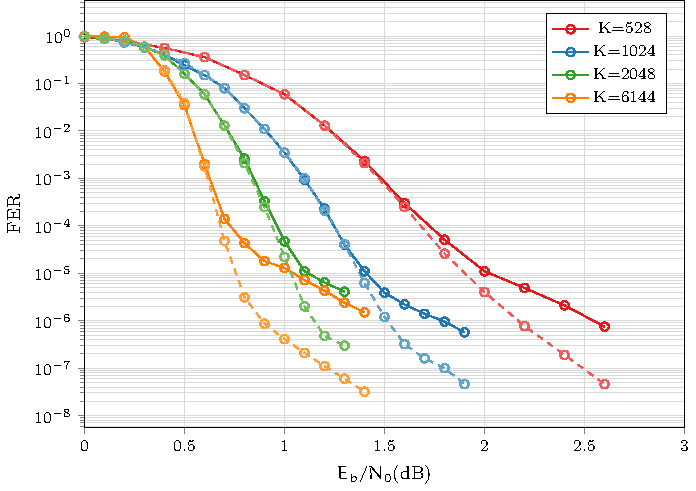
\includegraphics[width=\textwidth]{main/ch3_fig/fnc/lte/tikz/lte.pdf}
	\caption{Comparaison de performances de décodages entre EML-MAP et FNC. Standard LTE, K=528, 1024, 2048 et 6144. R=1/3.
	Décodeurs itérant jusqu'à 8 fois. \label{fig:fnc_lte}}
\end{figure}
Cette section présente des résultats de simulations Monte Carlo réalisées avec une représentation des données en 
virgule flottante.
Les tailles des trames considérées pour le standard LTE sont 528, 1024, 2048 et 6144. Dans tous les cas, le rendement
est fixé à 1/3. Afin d'éviter les problèmes de
faux positifs liés à l'emploi du code CRC de ce standard, la valeur de $I_\text{min}$ est fixée selon la 
taille de la trame de 2 à 5. Le processus
de turbo décodage peut itérer jusqu'à 8 fois. Enfin, la valeur de $q$ pour l'algorithme FNC est fixée à 10. La Figure 
\ref{fig:fnc_lte} présente une comparaison des performances entre un décodage utilisant l'algorithme EML-MAP avec critère 
d'arrêt sur code CRC (courbes en traits pleins) à un décodage basé sur l'algorithme FNC (courbes en pointillés).

Pour les quatre cas considérés, l'amélioration du processus de turbo décodage obtenu par l'algorithme FNC représente un
gain en terme de FER au moins égal à un ordre de grandeur dans la zone du plancher d'erreurs. Cela signifie qu'au moins 
$90\%$ des trames erronées sont corrigées par l'approche FNC. 
% Le Tableau \ref{tab:fnccomp} compare le taux d'erreur trame 
% attendu en extrapolant les performances de la métrique $\Delta_1$ présentée en section précédente et celui réellement obtenu avec 
% l'algorithme FNC pour $q=10$. Ces données proviennent de la Figure \ref{fig:idLTE}. 
% Cependant, comme le code CRC n'était à ce moment pas utilisé dans le décodage, il n'était pas comptabilisé dans le rendement. 
% Ce n'est pas le cas pour les courbes de la Figure \ref{fig:fnc_lte} où le code CRC est soit utilisé en tant que critère 
% d'arrêt, soit dans le processus FNC. Ainsi, pour pouvoir exploiter les données de la Figure \ref{fig:idLTE},
% un décalage de la valeur du SNR par $10\times \log_{10}\left(\frac{K}{K-24}\right)$
% doit leur être ajouté.
Puisque $q$ vaut 10, l'algorithme FNC ne peut corriger au maximum que 10 erreurs binaires. Au début de ce chapitre, la 
Figure \ref{fig:be} présentait le nombre d'erreurs binaires par trame erronée pour ces turbo codes. De là, il est possible 
d'extrapoler le taux d'erreur trame obtenu si l'ensemble des trames contenant 10 erreurs ou moins est corrigé. Ainsi, 
le tableau \ref{tab:fnccomp} présente ce taux d'erreur trame attendu et celui réellement observé avec l'algorithme de décodage
FNC et $q=10$. Il est à noter que lors de 
l'obtention des histogrammes de la Figure \ref{fig:be}, le code CRC n'était pas utilisé. Il n'était alors pas comptabilisé dans 
le rendement. En revanche, pour les données de la Figure \ref{fig:fnc_lte}, le code CRC est soit utilisé en tant que critère 
d'arrêt, soit dans le processus FNC. Un décalage de la valeur du SNR par $10\times \log_{10}\left(\frac{K}{K-24}\right)$
doit alors être considéré afin de pouvoir exploiter l'ensemble de ces données.
\begin{table}[]
\centering
\caption{Comparaison entre les valeurs de taux d'erreur trames attendues avec une correction parfaite et celui réellement obtenu}
\label{tab:fnccomp}
\begin{tabular}{@{}lrrrr@{}}
\toprule
    & \begin{tabular}[c]{@{}l@{}}\textbf{K=528}  \\ @ $2,6$ dB\end{tabular} & \begin{tabular}[c]{@{}l@{}}\textbf{K=1024} \\ @ $1,6$ dB\end{tabular} & \begin{tabular}[c]{@{}l@{}}\textbf{K=2048} \\ @ $1,35$ dB\end{tabular} & \begin{tabular}[c]{@{}l@{}}\textbf{K=6144} \\ @ $0,82$ dB\end{tabular} \\ 
    \cmidrule(l){2-2}\cmidrule(l){3-3}\cmidrule(l){4-4}\cmidrule(l){5-5}
FER EML-MAP (Fig. \ref{fig:fnc_lte})     & $7\times 10^{-7}$           & $2,3\times 10^{-6}$         & $3\times 10^{-6    }$         & $4\times 10^{-5    }$         \\
BE $\leq$ 10 (Fig. \ref{fig:be}) 		& $98\%$            & $94\% $           & $97\% $            & $97\%$           \\
FER attendu     & $1,4\times 10^{-8}$          & $1,4\times 10^{-7  }$        & $9\times 10^{-8     }$        & $1,2\times 10^{-6   }$          \\
FER FNC (Fig. \ref{fig:fnc_lte})        & $5\times 10^{-8 }$           &  $3\times 10^{-7  }$             & $2\times 10^{-7}$             & $2\times 10^{-6} $            \\ \bottomrule
\end{tabular}
\end{table}
% D'après ce tableau, il est visible que l'écart entre le taux d'erreur trame attendu et celui obtenu 
% est relativement faible. 
%Ceci démontre le choix judicieux réalisé précédemment dans le choix des valeurs de $I_\text{min}$.
%En effet, de la sorte, le code CRC n'a pas d'impact négatif sur la zone du plancher d'erreurs induit par les faux positifs.

À la vue des performances obtenues vis-à-vis de celles attendues, présentées dans le Tableau \ref{tab:fnccomp} nous pouvons statuer sur l'absence de 
dégradations due à d'éventuels faux positifs émanant de la détection via le code CRC. Ceci provient conjointement de sa
distance minimale suffisamment importante (provenant directement de sa taille) et de l'adaptation de $I_{\text{min}}$ en 
fonction de la taille de la trame.

Concernant le taux d'erreur binaire, les gains sont légèrement moins importants que ceux présentés pour le taux d'erreur trame. En effet,
de part son principe, l'algorithme FNC corrige les trames à faible nombre d'erreurs binaires. Ainsi, les trames erronées 
après processus FNC possèdent un nombre important d'erreurs binaires. Néanmoins, des gains d'environ un ordre de grandeur 
sont observés dans certains cas considérés. Ces résultats sont présentés en Annexe \ref{sec:ann3}.

La Figure \ref{fig:fnc_ccsds} présente les performances de l'algorithme FNC cette fois dans le contexte d'un turbo code 
du standard CCSDS. Les conditions sont les suivantes. La taille de la trame vaut 1784 et le rendement nominal R=1/3 est 
considéré. 
% Le turbo décodeur itère jusque 10 fois. Le code CRC définit dans le standard CCSDS possède une longueur de 16.
% Ainsi son pouvoir de détection d'erreurs est plus faible que celui du standard LTE. Aussi, les turbo codes du 
% standard CCSDS possèdent une longueur de contrainte de 5. 
% Cela implique que le nombre moyen d'itérations pour décoder une trame dans 
% la zone du plancher d'erreurs est plus élevé que dans le contexte LTE. Suite à ces deux constatations, la valeur de 
% $I_\text{min}$ se doit d'être plus élevée que précédemment. Elle est donc fixée à 5 afin de ne pas être limitée par le code CRC. 
Puisque les turbo codes du standard CCSDS possèdent une longueur de contrainte de 5, le nombre moyen d'itérations pour 
décoder une trame dans la zone du plancher d'erreurs est plus élevé que dans le contexte LTE. Aussi, le code CRC définit 
dans le standard CCSDS possède une longueur de 16. Ainsi son pouvoir de détection d'erreurs est plus faible que celui du 
standard LTE. Suite à ces deux constatations, la nombre maximal d'itérations est fixé à 10 et la valeur de $I_\text{min}$
est fixée à 5 afin que les performances de décodage ne soit pas limitées par le code CRC.

\begin{figure}[!hb]
	\centering
	\includegraphics[width=\textwidth]{main/ch3_fig/fnc/ccsds/tikz/ccsds.pdf}
	\caption{Comparaison de performances de décodages entre EML-MAP et FNC. Standard CCSDS, K=1784.
	Décodeurs itérant jusqu'à 10 fois. \label{fig:fnc_ccsds}}
\end{figure}

Il est visible sur la Figure \ref{fig:fnc_ccsds} que les gains sont légèrement moins importants que pour le standard LTE. 
Néanmoins, ces gains sont proches de l'ordre de grandeur.
Par cet exemple, nous entrevoyons une limite du principe FNC. En effet, si le code CRC définit par le standard considéré 
possède un risque important d'erreur non détectée, alors ce dernier est limitant dans les gains de décodage obtenu
avec l'algorithme FNC. \\
Une comparaison avec l'état de l'art portant sur la réduction de la zone du plancher d'erreurs 
par des approches basées sur un post-traitement est maintenant dressée.

\subsubsection{Positionnement par rapport à l'état de l'art}
\paragraph*{Performances de décodage}
Dans le chapitre premier, diverses méthodes permettant d'abaisser le plancher d'erreurs des turbo codes ont été présentées.
Il s'agit des méthodes FSM (ou CIM), de la concaténation en série d'un code BCH et enfin du décodage par liste. 
Les méthodes de décodages par listes et FSM sont dépendantes d'un code détecteur d'erreurs, comme le principe FNC. Ainsi, 
pour obtenir une comparaison cohérente, la courbe de référence correspond à un turbo code 
sans concaténation avec un code CRC, bien que celui-ci soit déjà présent dans la majorité de standards utilisant un turbo code. 
Ceci permet de ne pas désavantager l'approche considérant une concaténation avec un code BCH pouvant aussi agir comme 
code détecteur d'erreurs.

Dans \cite{cim}, les performances de décodage de la méthode CIM sont présentées en prenant pour cadre un turbo code ayant pour
polynôme générateur $(13,15)_8$. La taille de la trame vaut 1504. Le turbo décodeur implémente l'algorithme EML-MAP et
itère 16 fois. Cependant dans cette publication, la détection d'erreurs est réalisée par un génie. Cela signifie
que la décision du décodeur est comparée avec la trame émise. Afin de se positionner dans un contexte réaliste, le génie doit être remplacé
par un code CRC. Dans la Figure \ref{fig:fnc_soa}, nous considérons pour ce cas le code CRC du standard LTE, de taille 24 bits.
C'est pourquoi la courbe de performances associée à la méthode CIM est translatée vers la droite de $10\times\log_{10}\left(\frac{1504}{1504-24}\right)=0,07\text{ dB}$.
Pour des raisons de complexité calculatoire qui seront détaillées plus loin, seul le cas correspondant à un 
turbo décodage supplémentaire au maximum (CIM(1)) est considéré. Dans ce cas, les performances de cette méthode et celles de l'algorithme
FNC sont semblables.

Dans \cite{andersenBCH}, un code BCH est concaténé avec le turbo code dans le but de corriger les erreurs résiduelles 
après le processus de turbo décodage. Dans la Figure \ref{fig:fnc_soa}, les performances associées à cette technique sont
reportées. La capacité de 
correction d'un code BCH est directement donnée par la quantité d'information redondante (\textit{cf.} premier chapitre). Or, cet 
ajout abaisse le rendement du schéma de codage. En résulte alors un décalage de la courbe de performance dans la zone de convergence 
vers la droite. Deux codes BCH différents sont testés : l'un corrigeant toutes les trames contenant 4 erreurs ou moins (t=4), l'autre 
corrigeant celles contenant 10 erreurs ou moins (t=10). Dans le premier cas, les performances dans la zone du plancher 
d'erreurs sont moins intéressantes que celles obtenues par l'algorithme FNC. Il faut en effet que le code BCH ait un pouvoir
de correction de 10 pour obtenir les mêmes performances que l'algorithme FNC dans la zone du plancher d'erreurs. Cependant, 
dans ce cas, la pénalité de convergence vaut $0,33$ dB. Son utilisation dans un contexte de communications numériques 
est alors compromise. L'emploi d'un tel code concaténé peut néanmoins avoir un intérêt pour des tailles de trames
conséquentes. En effet la taille de l'information redondante est liée au logarithme en base 2 de la taille de trame.
C'est la raison pour laquelle un tel schéma a été choisi avec le code LDPC du standard DVB-S2.

\begin{figure}[!htb]
	\centering
	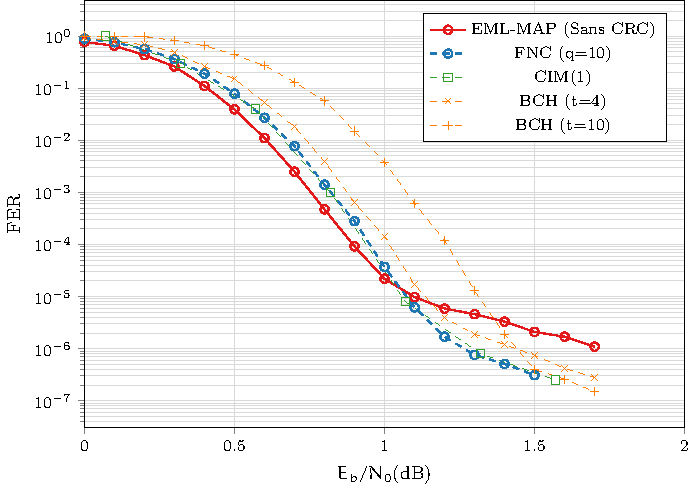
\includegraphics[width=\textwidth]{main/ch3_fig/fnc/soa/tikz/soa.pdf}
	\caption{Comparaison de performances de décodages entre EML-MAP, FNC, CIM et concaténation avec BCH. K=1504 et générateur
	polynomial $(13,15)_8$.	Décodeurs itérant jusqu'à 16 fois. \label{fig:fnc_soa}}
\end{figure}

\paragraph*{Complexité calculatoire} Selon \cite{david_gnaedig_thesis}, les calculs nécessaires pour qu'un turbo décodeur 
effectue une itération de l'algorithme EML-MAP pour un turbo code à 8 états s'établissent à $130\times K$ additions 
et $62\times K$ opérations de comparaison et sélection.

Pour chaque itération, l'algorithme FNC est basé sur deux opérations principales. Tout d'abord, il s'agit de l'extraction 
des positions les moins fiables. Ceci peut être réalisé par un tri par insertion. Il nécessite alors $(K-q)\times q$ 
opérations de comparaison. Ensuite les $2^q$ vérifications du code CRC doivent avoir lieu. 
% Pour implémenter chacune de ces vérifications,
% dans le cas du standard LTE, 24 bascules D sont nécessaires ainsi que 13 portes ou-exclusif. 
Néanmoins, chacune de ces vérifications peut correspondre à une opération élémentaire.
De la sorte, même si le 
nombre de calculs de CRC croit exponentiellement avec $q$, il reste relativement faible en comparaison du nombre 
d'opérations nécessaires à chaque itération du turbo décodeur. 
Aussi, il est à noter que l'approche FNC n'est pas à proprement parler un algorithme 
de post-traitement. En effet, son application sur les données produites par le turbo décodeur à l'itération $i$ peut être 
envisagé lors de l'itération $i+1$.  De la sorte, il n'impacte que peu la latence du système. Cette notion sera développée 
en détail dans le prochain chapitre.

L'approche CIM(1) repose sur l'emploi de deux processus de turbo décodage successifs. Sa complexité calculatoire est donc
égale à deux fois celle d'un turbo décodage classique. A cela, il faut rajouter un tri des valeurs, qui est 
le même que pour l'algorithme FNC. En revanche, ce tri n'est effectué qu'une seul fois par trame alors que dans le cas de l'algorithme
FNC il est effectué après chaque itération. En ce qui concerne la latence, la méthode CIM ne 
peut effectuer le post-traitement qu'après la fin du premier processus de décodage. Elle impacte alors fortement la latence
maximale du système. Ce qui n'est pas le cas de l'approche FNC.

Enfin, en ce qui concerne la concaténation avec un code BCH, le décodage de ce dernier est basé sur un calcul 
de syndrome et  l'emploi de l'algorithme
de Berlekamp-Massey suivi pas celui de Chien. Ces algorithmes reposent sur des additions et multiplications dans un corps
de Galois $GF(2^{\log_2 K})$, qui possèdent une complexité calculatoire relativement importante. Aussi, quelques additions
et opérations de comparaison et sélection sont nécessaires (respectivement $t\times K$ et $6t\times K$). 

Le Tableau \ref{tab:cplx_soa_th} récapitule les valeurs formelles des opérations à réaliser pour ces différentes approches.
Le Tableau \ref{tab:cplx_soa} correspond aux applications numériques pour un turbo code 8 états avec K=1504 et 
R=1/3 et un processus de décodage itérant 16 fois (contexte de la Figure \ref{fig:fnc_soa}). A la vue des performances de 
décodage obtenues et de sa complexité calculatoire, l'algorithme FNC se compare favorablement aux approches de réduction
du plancher d'erreurs des turbo codes.

\begin{table}[!t]
    \centering
    \caption{Comparaison de la complexité calculatoire pour les différentes approches de post-traitement des turbo codes, valeurs théoriques}
    \label{tab:cplx_soa_th}
    \resizebox{\linewidth}{!}{
        \begin{tabular}{rllll}
            \toprule
            				& TDec 				& TDec + FNC 								& TDec + CIM(1) 		& TDec + BCH 					\\
            \cmidrule(l){2-2}\cmidrule(l){3-3}\cmidrule(l){4-4}\cmidrule(l){5-5}
            Add 			& $130.K.I_{TC}$	& $K(130.I_{TC} + I_{TC}-I_{min})$			& $2.130.K.I_{TC} + K$	& $K(130.I_{TC} + t)$			\\
            CS  			& $62.K.I_{TC}$	& $K(62.I_{TC} + q\left(I_{TC}-I_{min})\right)$ & $2.62.K.I_{TC} + K$	& $K(62.I_{TC} + 6.t)$			\\
            CRC 			& $I_{TC}-I_{min}$  & $2^q.(I_{TC}-I_{min})$ 					& $2(I_{TC}-I_{min})$ 	& $0$	  						\\
Add GF$\left(2^{11}\right)$ & $0$ 				& $0$										& $0$					& $K(t-1)+t^2$					\\
Mul GF$\left(2^{11}\right)$ & $0$				& $0$										& $0$					& $2.t.K + \frac{3.t(t+1)-4}{2}$\\
            \bottomrule
        \end{tabular}}
\end{table}


\begin{table}[!t]
    \centering
    \caption{Comparaison de la complexité calculatoire pour $K=1504$, $I_{TC}=16$, $I_{min}=3$, $q=10$ et $t=10$ }
    \label{tab:cplx_soa}
    %\resizebox{\linewidth}{!}{
        \begin{tabular}{rllll}
            \toprule
            		& TDec 			& TDec + FNC 	& TDec + CIM(1) & TDec + BCH \\
            \cmidrule(l){2-2}\cmidrule(l){3-3}\cmidrule(l){4-4}\cmidrule(l){5-5}
            Add 	& $3~128~320$ 	& $3~143~360$ 	& $6~258~144$ 	& $3~143~360$ \\
            CS  	& $1~491~968$ 	& $1~642~368$ 	& $2~985~440$ 	& $1~582~208$ \\
            CRC 	& $13$      	& $13~312$   	& $26$      	& $0$       \\
            Add GF$\left(2^{11}\right)$ & $0$ & $0$ &$0$			& $13~636$ \\
            Mul GF$\left(2^{11}\right)$ & $0$ & $0$ &$0$			& $30~243$ \\
            \bottomrule
        \end{tabular}%}
\end{table}

\subsubsection{Conclusions}
L'algorithme Flip and Check pour les turbo codes binaires a été présenté. Celui-ci permet d'abaisser le plancher d'erreurs 
des turbo codes binaires d'au moins une décade. Ses performances sont proches de celles atteignables via une 
identification parfaite. La complexité calculatoire de cet algorithme réside dans les vérifications du code CRC. Cette 
complexité croit exponentiellement avec le nombre de positions les moins fiables considérées. Toutefois, une 
comparaison avec l'état de l'art a montré que son surcoût calculatoire est raisonnable tout en fournissant de très bonnes 
performances de décodage. Finalement, cette méthode peut s'adapter à des turbo codes standardisés dès lors qu'un code 
détecteur d'erreurs, comme un code CRC, y est concaténé en série. Ce travail à fait l'objet d'une publication dans revue
internationale avec comité de lecture \citemine{wcl}. Dans la suite, une adaptation aux turbo codes double binaires est détaillée.


\subsection{Application aux turbo codes double binaires}
Cette section propose une transposition de l'algorithme FNC au cas des turbo codes double binaires. Après avoir décrit 
les transformations nécessaires, l'algorithme adapté aux turbo codes double binaires est exprimé. Enfin, une présentation 
des performances obtenues est réalisée.
\subsubsection{Identification des symboles les moins fiables}
Lors de la comparaison des métriques d'identification effectuée au début de ce chapitre, plusieurs propositions ont été 
comparées. L'une d'entre elles, la métrique $\Delta'_1$, possède les meilleures performances d'identification. C'est donc
celle qui est retenue pour la transposition au cas double binaire. Cependant, dans le cas double binaire, les positions identifiées correspondent 
à des symboles double binaires. Chaque position représente alors 4 symboles différents. Suivant cette constatation, une adaptation directe 
requerrait la génération de $4^q$ mots candidats. Le nombre de vérifications du code CRC ayant la même valeur, 
seules de faibles valeurs de $q$ pourraient être considérées. Or, d'après les statistiques d'identification présentées en Figure 
\ref{fig:dvb752}, afin de pouvoir observer une amélioration notable des performances de décodage, le choix de $q$ implique 
de se porter \textit{a minima} à 8 afin de corriger $80\%$ des trames erronées dans la zone du plancher d'erreurs. Dans 
ce cas, 65536 vérifications de CRC seraient nécessaires, ce qui est 
irréaliste dans un contexte temps réel visant une faible complexité.

C'est pourquoi, il est nécessaire de réduire le nombre de symboles testés par position identifiée. Pour ce faire, une 
analyse a été menée quant à l'identification du bon symbole à l'aide d'un critère génie. Cette identification est semblable 
à celle permettant l'extraction des positions les moins fiables.
Soient $S_{M_x}(k)$, $S_{M_y}(k)$, $S_{M_z}(k)$, et $S_{M_t}(k)$ respectivement le symbole le plus probable au sens 
des informations \textit{a posteriori}, le second symbole le plus probable, le troisième et enfin le symbole le moins 
probable. Ils ont alors pour expression :
\begin{align*}
S_{M_x}(k) &= \argmax\limits_{s\in\llbracket0;3\rrbracket}\left(l^a_s(k)\right) \\
S_{M_y}(k) &= \argmax\limits_{s\in\llbracket0;3\rrbracket\setminus{S_{M_x}(k)}}\left(l^a_s(k)\right)\\
S_{M_z}(k) &= \argmax\limits_{s\in\llbracket0;3\rrbracket\setminus{\{S_{M_x}(k)}, S_{M_y}(k)\}}\left(l^a_s(k)\right)\\
S_{M_t}(k) &= \{0,1,2,3\}\setminus{\{S_{M_x}(k), S_{M_y}(k), S_{M_z}(k)\}}
\end{align*}
Le tableau \ref{tab:symb} présente des statistiques quant au symbole réellement transmis en fonction des valeurs 
\textit{a posteriori} associées à ce symbole lorsqu'il est erroné à l'issue de l'itération courante. 
Ces statistiques ont été obtenues pour différents turbo codes du standard DVB-RCS. 
Cela permet de déduire les symboles à considérer lors de la génération des 
mots candidats. Nous pouvons constater que la première colonne vaut toujours 0\% puisque le symbole le plus probable correspond au
symbole décodé. 
Cependant, si pour obtenir $S_{M_\xi}$ l'information \textit{a posteriori} doit être reconstruite 
(cas où le décodeur SISO fournit en sortie l'information extrinsèque et le vecteur décidé), il est important de ne pas 
ommetre le facteur de remise à l'échelle. En effet, l'identification via la métrique $\Delta'$ est correct
en raison du faible écart entre les valeurs \textit{a posteriori}. Ainsi, une légère modification dans leurs calculs 
modifie grandement la trame décodée. Il serait alors possible d'aboutir à ce que le symbole le plus probable estimé ne
soit pas celui décodé.
\begin{table}[!tb]
    \centering
    \caption{Statistiques sur le symbole transmis vis-à-vis des différents symboles possibles}
    \label{tab:symb}
    %\resizebox{\linewidth}{!}{
        \begin{tabular}{lrrrr}
            \toprule
            		& $S_{M_x}$	& $S_{M_y}$	& $S_{M_z}$ & $S_{M_t}$ \\
            \cmidrule(l){2-2}\cmidrule(l){3-3}\cmidrule(l){4-4}\cmidrule(l){5-5}
            i=3     &	0\%		&	96\%	& 	3\%		&	1\%		\\
            i=4     &	0\%		&	96\%	& 	3\%		&	1\%		\\
            i=5     &	0\%		&	97\%	& 	3\%		&	0\%		\\
            i=6     &	0\%		&	97\%	& 	3\%		&	0\%		\\
            i=7     &	0\%		&	97\%	& 	3\%		&	0\%		\\
            i=8     &	0\%		&	97\%	& 	2\%		&	1\%	\\
            \bottomrule
        \end{tabular}%}
\end{table}
 
À la lecture du tableau, il apparaît que dans la très grande majorité des cas, le symbole transmis 
correspond au symbole le deuxième plus probable. Cela implique que considérer plus que deux symboles ne 
permet alors pas d'augmenter de manière significative la probabilité de fournir le bon mot de code alors que la complexité 
calculatoire résultante serait tout à fait notable.

Finalement, de part cette analyse, considérer uniquement les deux symboles les plus probables est suffisant pour 
pouvoir identifier dans la plupart des cas le bon mot de code. Le nombre de vérifications de code CRC reste alors 
équivalent au cas binaire et vaut $2^q$. Une étape supplémentaire consistant à l'extraction des deux symboles les plus probables est néanmoins 
nécessaire. Dès lors, il est possible de proposer l'algorithme complet, sujet de la prochaine sous-section.

\subsubsection{Détail de l'algorithme pour les turbo codes double binaires}
L'algorithme FNC pour les turbo codes double binaires est très similaire à celui du cas binaire. Seules quelques 
opérations supplémentaires s'avèrent nécessaires. Il peut être détaillé comme suit. Tout d'abord, $I_{\text{min}}$ itérations de 
turbo décodages seuls sont effectuées. Ceci permet de réduire le risque de faux positifs lié à l'utilisation 
d'un code CRC. À partir de l'itération suivante, le code CRC commence à être vérifié. S'il ne l'est pas, le principe FNC
est alors appliqué. D'abord, pour chaque position symbole dans la trame, les deux symboles les plus probables sont 
extraits au sens de l'information \textit{a posteriori}. Ceci permet de calculer la métrique $\Delta'_1$. Une fois que 
tous ses indices ont été calculés, les $q$ positions des symboles les moins fiables sont extraites en triant par ordre 
croissant la métrique $\Delta'_1$. Ces positions sont stockées dans le vecteur $\Omega$. Ensuite, à partir des positions contenues dans
$\Omega$ et des indices de $S_{M_x}$ et $S_{M_y}$, les valeurs des deux symboles les plus probables sont extraites pour 
chacune des positions présupposées erronées. Il reste ensuite à générer les $2^q$ mots candidats en remplaçant la valeur des symboles
aux positions correspondantes dans le mot produit à cette itération. Finalement, ces mots candidats sont vérifiés
en utilisant le code CRC. Si un mot de code est trouvé, alors le processus itératif est stoppé. Sinon, une nouvelle itération
du processus de turbo décodage est effectuée. L'algorithme \ref{alg:fc_db} récapitule l'ensemble de ces opérations.

Dans le contexte de turbo codes double binaires, l'algorithme FNC nécessite donc plus d'opérations que dans le cas binaire.
Ceci provient directement de la manipulation de symboles. Cependant, l'opération d'extraction nécessaire des deux symboles 
les plus probables correspond à une manipulation pour l'hypothétique correction de deux bits. Dès lors, la complexité globale
de l'algorithme par bit décodé n'est que peu modifiée.\\
Ces deux extractions de valeurs maximales correspondant aux lignes 9, 10 et 13 de l'algorithme \ref{alg:fc_db}) 
correspondent à un tri entre 4 valeurs.
% Afin de réaliser ces deux extractions de valeurs maximales (correspondant aux lignes 9, 10 et 13 de l'algorithme 
% \ref{alg:fc_db}), un réseau de tri doit être utilisé. Dans ce cas, pour chaque symbole, 5 comparaisons sont nécessaires.
% En utilisant la décision du turbo décodeur, il serait possible de réduire le nombre de comparaison à 3. Mais dans ce cas,
% de la logique combinatoire supplémentaire sera nécessaire afin de sélectionner les entrées de ces 3 comparateurs. 
Comme ces opérations
ne sont réalisées qu'une fois par itération, leur impact sur la complexité calculatoire globale reste faible. Dans la suite de 
cette sous-section, une présentation
des performances de décodage dans le contexte des standards DVB-RCS et DVB-RCS2 est réalisée.\vspace*{-1em}
\begin{center}
\begin{minipage}{.95\textwidth}%
\begin{algorithm}[H]
\label{alg:fc_db}
	\DontPrintSemicolon
	\SetKwFunction{TD}{Itération de Turbo Décodage}
	\SetKwFunction{GC}{Génération du mot candidat}
	\SetKwFunction{L}{Extraction des positions des symboles les moins fiables}
	\SetKwFunction{S}{Extraction des 2 symboles les plus fiables}
	\SetKwFunction{R}{return}
	\SetKwFunction{CRC}{CRCheck}
	
	\For{i: 1 à  $I_{min}$}{
		\TD\;
	}
	\For{i: $I_{min}+1$ to  $I_{TC}$}{
		$\left(\mathbf{\hat{{d}}}, \mathbf{L}\right)$ = \TD\;
		\If{\CRC{$\mathbf{\hat{{d}}}$}==true}{
			\R{$\hat{{d}}$}\;
		}
		\Else{
			\For{k: 1 à K}{	
				$S_{M_x}(k) = \argmax\limits_{s\in\llbracket0;3\rrbracket}\left(l^a_s(k)\right)$\;
				$S_{M_y}(k) = \argmax\limits_{s\in\llbracket0;3\rrbracket\setminus{S_{M_x}(k)}}\left(l^a_s(k)\right)$\;
				$\Delta'_k = l^a_{S_{M_x}}(k)-l^a_{S_{M_y}}(k)$\;		%
			}
			$\Omega =$ \L{$\Delta$, q}\;
			$\xi =$ \S{$\Omega$, $S_{M_x}$, $S_{M_y}$}\;
			\For{j: 1 à $2^q-1$}{								
				$\mathbf{D} =$\GC{$\Omega, \xi, j, \mathbf{\hat{d}}$}\;
				\If{\CRC{$\mathbf{D}$}==true}{
					\R{$\mathbf{D}$}\;
				}
			}
		} %end else
	}
	\R{$\hat{{d}}$}\;
	\caption{L'algorithme Flip and Check pour les turbo codes double binaires}
\end{algorithm}
\end{minipage}
\end{center}


\subsubsection{Performances de décodage}
Dans cette section les résultats de simulations Monte Carlo réalisées avec une représentation des données en virgule
flottante sont détaillés. Un canal AWGN est toujours considéré. En revanche, la modulation numérique est maintenant une QPSK. Le 
nombre maximum d'itérations réalisées par le turbo décodeur est fixé à 8 et $I_{\text{min}}$ vaut 3.
Comme dans le cas binaire, la valeur de $q$ est fixée à 10. Dans le standard DVB-RCS, les tailles de trame sont comprises
entre quelques dizaines d'octets et 200 octets. Sept rendements différents sont définis allant de 1/3 à 6/7. Le code CRC 
considéré dans ce standard est de longueur 16. La Figure \ref{fig:fnc_dvb1_440} compare les performances du turbo décodage
conventionnel avec celles de l'algorithme FNC pour K=440 symboles et pour différentes valeurs de rendement. 
% Il apparaît 
% ainsi que grâce à l'algorithme FNC, dans la zone du plancher d'erreurs, le turbo code de rendement 1/2 possède de 
% meilleures performances que celles obtenues pour le turbo code de rendement 1/3 avec un décodage conventionnel EML-MAP. 
% Plus généralement, pour des valeurs de SNR moyennes à élevées, quelque soit le rendement du code, l'algorithme FNC apporte 
% des gains au moins égaux à un ordre de grandeur. 
Il apparaît que grâce à l'algorithme FNC, dans la zone du plancher d'erreurs, quelque soit le rendement du code, l'algorithme FNC apporte 
des gains au moins égaux à un ordre de grandeur. 
En terme de SNR, cela correspond à des gains allant de $0,4$ dB à plus de 
$0,6$ dB.

Pour les autres tailles de trame du standard, les gains sont tout aussi conséquents. Pour confirmer ces
dires, des courbes de performance présentant le taux d'erreur trame obtenu avec l'algorithme FNC pour $K=752$ sont fournies en 
Annexe \ref{sec:ann3}. En résumé, il apparaît que la pente de la courbe dans la zone du plancher d'erreurs est modifiée, l'inflexion
est moins importante grâce à l'algorithme FNC.

\begin{figure}[!t]
	\centering
	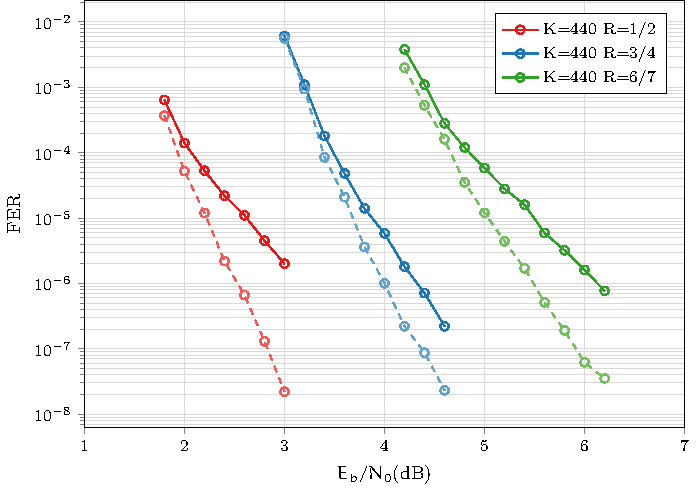
\includegraphics[width=\textwidth]{main/ch3_fig/fnc/dvb/tikz/dvb1_440.pdf}
	\caption{Comparaison des performances de décodage entre EML-MAP et FNC. Standard DVB-RCS, K=440, rendements de 1/2 à 
	6/7. Décodeurs itérant jusqu'à 8 fois. \label{fig:fnc_dvb1_440}}
\end{figure}
En 2012, la deuxième version du standard DVB-RCS a été publiée. Le code correcteur considéré est toujours un turbo code double
binaire. En revanche, afin d'améliorer les performances de correction, la longueur de contrainte des codes constituants
est augmentée. Des turbo codes à 16 états sont alors proposés. Un nouvel entrelaceur ARP ainsi que des tailles de trame
plus conséquentes sont également retenus. La taille du code CRC concaténé en série double, pour passer à une taille de 32 bits. 
Enfin, de nouveaux schémas de poinçonnage sont ajoutés. De la sorte, ces turbo codes font 
partis des codes correcteurs les plus performants et flexibles standardisés. La complexité calculatoire de ce code a
toutefois doublé en comparaison avec celle du turbo code de la génération précédente. 

\begin{figure}[!htb]
	\centering
	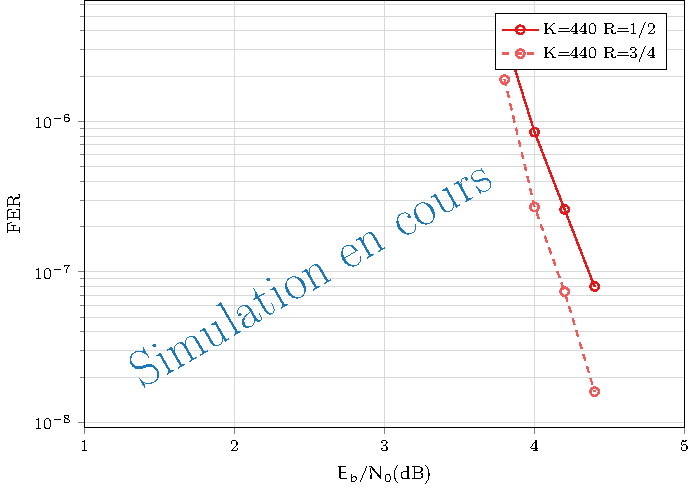
\includegraphics[width=\textwidth]{main/ch3_fig/fnc/dvb2/tikz/dvb2.pdf}
	\caption{Comparaison de performances de décodages entre EML-MAP et FNC. Standard DVB-RCS 2, K=752, Rendement de 1/2 à 
	4/5. Décodeurs itérant jusqu'à 8 fois. \label{fig:fnc_dvb2_752}}
\end{figure}

La Figure \ref{fig:fnc_dvb2_752} présente une comparaison des performances de décodage pour le standard DVB-RCS 2 avec
K=752. Différents rendements sont considérés : 1/2, 2/3, 3/4 et 4/5. Les autres paramètres de la simulation restent les
mêmes que pour le cas 8 états.
Tout d'abord, en considérant un décodage conventionnel, il apparaît que les performances de ce code surpassent très largement 
celles du DVB-RCS. En effet, les points d'inflexions des différentes courbes de performance apparaissent 2 à 3 décades
plus bas. La zone du plancher d'erreurs correspond alors à des taux d'erreur trame de l'ordre de $10^{-7}$. Ceci entraîne
un temps conséquent pour les simulations Monte-Carlo. De plus, comme l'algorithme FNC vise à abaisser le plancher 
d'erreurs, apercevoir une trame erronée devient alors extrêmement rare. Ainsi les courbes obtenues ne comptent que 30 
trames erronées avec l'algorithme de décodage FNC.

Il apparaît que même dans un contexte de turbo code très performants, des gains conséquents dans la zone du plancher d'erreurs 
sont obtenus grâce à l'emploi de l'algorithme FNC. À nouveau, un changement de la pente de la courbe dans cette zone est
visible. Ceci a pour conséquence de fournir des gains approchant la décade dans certains cas comme pour R=4/5. Dans d'autres
cas, comme pour R=1/2, les gains atteignent l'ordre de grandeur. Ce travail a fait l'objet d'une publication en
conférence internationale avec acte \citemine{symp1}.

\section{Conclusion}
Dans ce troisième chapitre, une étude sur les erreurs résiduelles des turbo codes a été menée. Dans un premier temps,
leur existence a été caractérisée grâce aux spectres de distances des turbo codes. Ces erreurs étant responsables de 
la zone du plancher d'erreurs, des propositions de critères d'identifications ont alors été comparées.

Cette comparaison a permis de mettre en exergue une métrique, permettant d'identifier de façon quasi-systématique
les erreurs résiduelles à l'issue du processus de turbo décodage. À partir de celle-ci, un algorithme, nommé Flip and Check
a été proposé. Cet algorithme tire parti de l'augmentation de la distance minimale obtenue via la concaténation en série 
d'un code détecteur d'erreurs et d'un turbo code. Un tel schéma de codage est couramment rencontré dans les standards de 
communications numériques. Le principe de cet algorithme repose sur l'identification des positions les moins fiables dans la séquence en train 
d'être décodée. De là, différents mots de code candidats sont générés puis vérifiés en utilisant le code détecteur d'erreurs.
Des gains d'au moins un ordre de grandeur ont été observés, ce, quelque soit le turbo code standardisé considéré. Ainsi, des gains
de performances conséquents sont observables pour des turbo codes binaires à 8 ou 16 états ainsi que pour des turbo codes 
double binaires eux aussi à 8 ou 16 états. La complexité calculatoire additionnelle nécessaire à cet algorithme est modérée,
comme le montre l'analyse de complexité calculatoire.
Cela rend cette approche compétitive par rapport à l’état de l'art sur la réduction du plancher d'erreurs des turbo codes.

Dans le chapitre suivant, après une étude des architectures matérielles de turbo décodeurs, des propositions d'implémentation 
de l'algorithme Flip and Check sont détaillées.


% Conclusion: Méthode relativement simple à mettre en oeuvre qui tire parti de l'auigmentation de la dmin du code grace a 
% la concat.
%PAS DE SPECTRE EN DOUBLE BINAIRE...
%CONFIRMER VALEURS TABLEAU FNC
%Gains obtenables par la méthode dépendent de la distribution de spectre d'erreur

%Parler métriques aposteriori binaires pour le double binaire => non présentées car moins performantes